\documentclass[a4paper,11pt]{article}
\usepackage[onehalfspacing]{setspace} %Zeilenabstand
\addtolength{\hoffset}{-2.25cm}
\addtolength{\textwidth}{4.5cm}
\addtolength{\voffset}{-3.25cm}
\addtolength{\textheight}{5cm}
\setlength{\parskip}{0pt}
\setlength{\parindent}{0in}

%----------------------------------------------------------------------------------------
%	PACKAGES AND OTHER DOCUMENT CONFIGURATIONS
%----------------------------------------------------------------------------------------

\usepackage{blindtext} % Package to generate dummy text
\usepackage{charter} % Use the Charter font
\usepackage[utf8]{inputenc} % Use UTF-8 encoding
\usepackage{microtype} % Slightly tweak font spacing for aesthetics
\usepackage[english, ngerman]{babel} % Language hyphenation and typographical rules
\usepackage{amsthm, amsmath, amssymb} % Mathematical typesetting
\usepackage{float} % Improved interface for floating objects
\usepackage[final, colorlinks = true, 
            linkcolor = black, 
            citecolor = black]{hyperref} % For hyperlinks in the PDF
\usepackage{graphicx, multicol} % Enhanced support for graphics
\usepackage{xcolor} % Driver-independent color extensions
\usepackage{marvosym, wasysym} % More symbols
\usepackage{rotating} % Rotation tools
\usepackage{censor} % Facilities for controlling restricted text
\usepackage{listings, style/lstlisting} % Environment for non-formatted code, !uses style file!
\usepackage{pseudocode} % Environment for specifying algorithms in a natural way
\usepackage{style/avm} % Environment for f-structures, !uses style file!
\usepackage{booktabs} % Enhances quality of tables
\usepackage{tikz-qtree} % Easy tree drawing tool
\tikzset{every tree node/.style={align=center,anchor=north},
         level distance=2cm} % Configuration for q-trees
\usepackage{style/btree} % Configuration for b-trees and b+-trees, !uses style file!
\usepackage{csquotes} % Context sensitive quotation facilities
\usepackage[yyyymmdd]{datetime} % Uses YEAR-MONTH-DAY format for dates
\renewcommand{\dateseparator}{-} % Sets dateseparator to '-'
\usepackage{fancyhdr} % Headers and footers
\pagestyle{fancy} % All pages have headers and footers
\fancyhead{}\renewcommand{\headrulewidth}{0pt} % Blank out the default header
\fancyfoot[L]{} % Custom footer text
\fancyfoot[C]{} % Custom footer text
\fancyfoot[R]{\thepage} % Custom footer text
\newcommand{\note}[1]{\marginpar{\scriptsize \textcolor{red}{#1}}} % Enables comments in red on margin

%----------------------------------------------------------------------------------------

\usepackage[english]{babel}
\usepackage{shellesc}
\usepackage{csquotes}
\usepackage[T1]{fontenc}
\usepackage{lmodern}
\usepackage{listings}
\usepackage{hyperref}
\usepackage[style=apa, backend=biber]{biblatex}
\addbibresource[]{ref.bib}
\renewcommand{\qed}{\hfill\blacksquare}
\newcommand{\qedwhite}{\hfill \ensuremath{\Box}}
\definecolor{answercolor}{HTML}{0071BC}
\newcommand*{\answer}{\textcolor{answercolor}}
\newenvironment{answerenv}{\color{answercolor}}{}
\newcommand{\E}{\mathbb{E}}
\usepackage{booktabs}
\usepackage{longtable}
\setcounter{section}{-1}

\begin{document}
\selectlanguage{english}
%-------------------------------
%	TITLE SECTION
%-------------------------------

\fancyhead[C]{}
\hrule  % Upper rule
\begin{minipage}{0.295\textwidth} 
\raggedright
\footnotesize
Lucas Paul Unterweger \hfill\\   
\hfill\\
Sophia Oberbrinkmann
\end{minipage}
\begin{minipage}{0.4\textwidth} 
\centering 
\large 
Assignment 1\\ 
\normalsize 
Adv. Macro II\\ 
\today \\
\end{minipage}
\begin{minipage}{0.295\textwidth} 
\raggedleft

\includegraphics[scale=0.15]{style/wu_transparent.png}\\
\end{minipage}
\hrule 
\bigskip

%-------------------------------
%	CONTENTS
%-------------------------------
\section{Preliminary}
We hereby declare that the answers to the given assignment are entirely our own, resulting from our own work effort only. Our team members contributed to the answers of the assignment in the following proportions: Unterweger Lucas: 50\%, Oberbrinkmann Sophia: 50\%

\tableofcontents

\subsection{Signatures}
\pagebreak
\listoffigures
\pagebreak
\section{Business cycle stylized facts (4 points)}
For this question, we chose to use data from \textbf{Ireland}. Before starting the analysis, we'll provide a short sample of the data set we gathered from \textit{EUROSTAT}.

\begin{figure}[h]
    \centering
    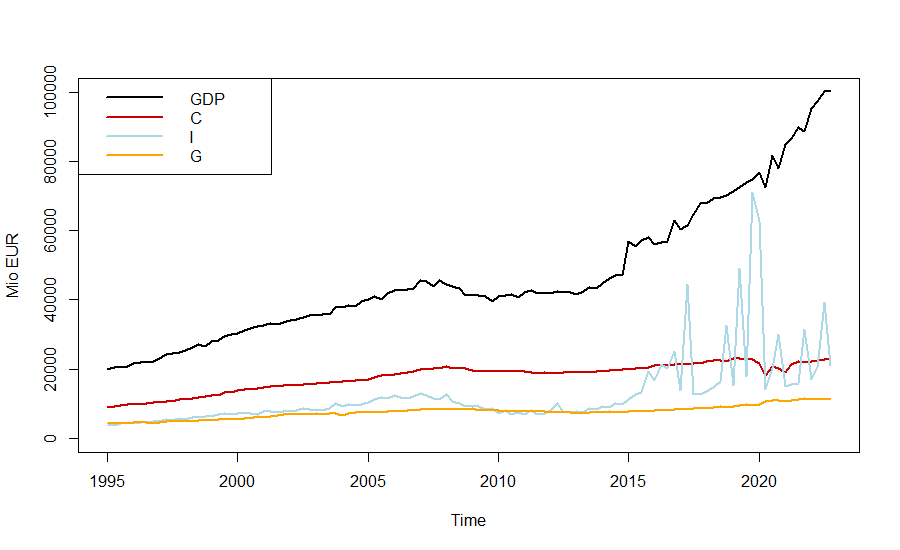
\includegraphics[scale=0.7]{rawdataplot_ireland.png}
    \caption{GDP, Investment, Consumption and State Expenditures of Ireland in Mio EUR}
    \label{fig:rawdata}
\end{figure}

The sample means of $C/Y$, $I/Y$ and $G/Y$ are the following:
\begin{longtable}[c]{@{}ll@{}}
\toprule
Sample Mean of    & Value    \\* \midrule
\endfirsthead
\endhead
\bottomrule
\endfoot
\endlastfoot
$C/GDP$ & $0.4063485$\\
$I/GDP$ & $0.2530171$\\
$G/GDP$ & $0.1719054$ \\* \bottomrule
\end{longtable}

To obtain the stationary (cyclical) component of these macroeconomic time series we are going to apply HP-filtering to the logged time series. To compute these using R, we will use the \textit{mFilter} package. The resulting plots are given below:
\begin{figure}[H]
    \centering
    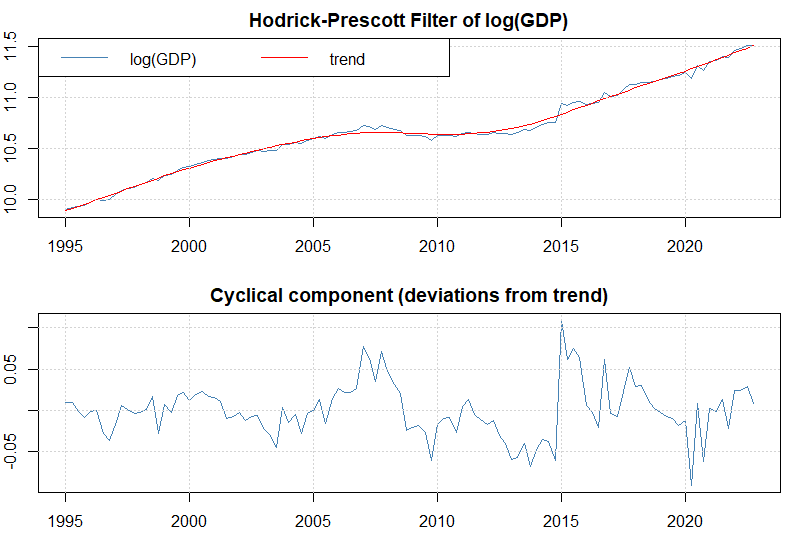
\includegraphics[scale=0.65]{HPFilter_GDP.png}
    \caption{HP Filter applied to logged GDP}
    \label{fig:my_label}
\end{figure}

\begin{figure}[H]
    \centering
    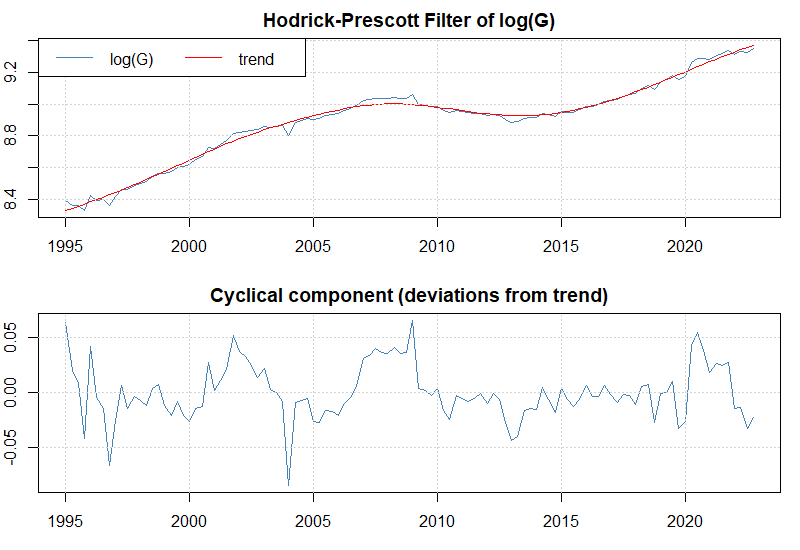
\includegraphics[scale=0.65]{HPFilter_G.png}
    \caption{HP Filter applied to logged G}
    \label{fig:my_label}
\end{figure}
\begin{figure}[H]
    \centering
    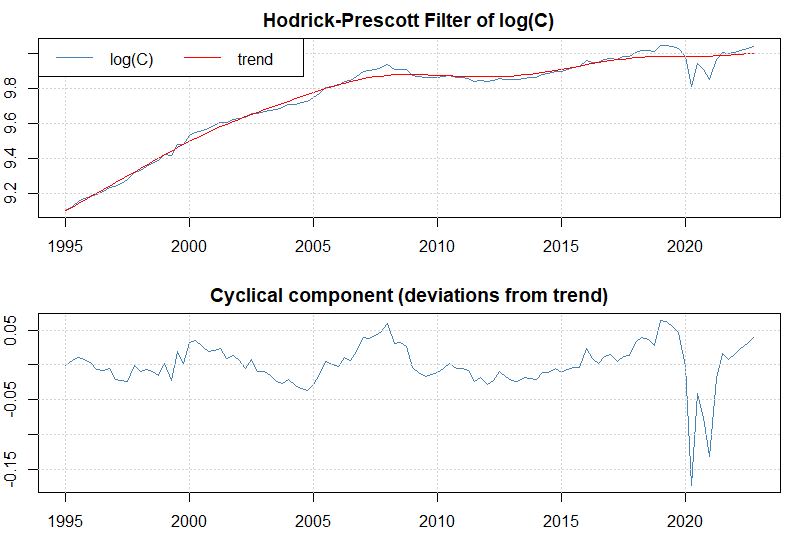
\includegraphics[scale=0.65]{HPFilter_C.png}
    \caption{HP Filter applied to logged C}
    \label{fig:my_label}
\end{figure}
\begin{figure}[H]
    \centering
    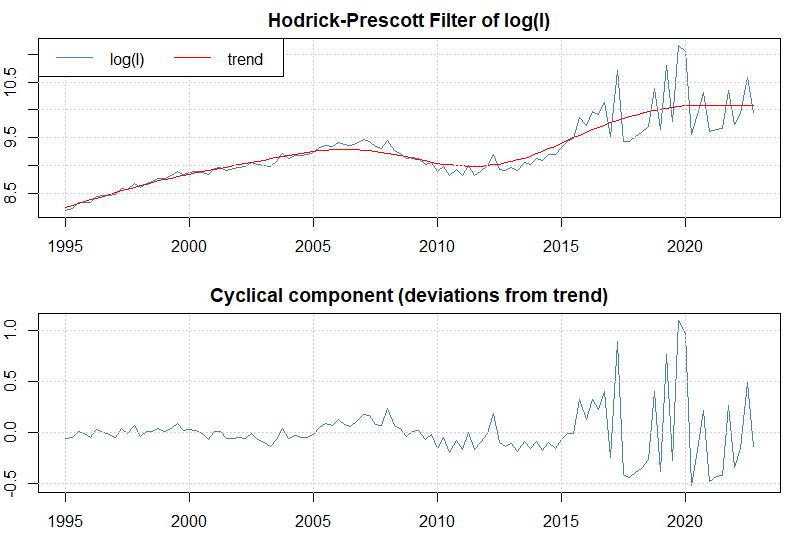
\includegraphics[scale=0.65]{HPFilter_I.png}
    \caption{HP Filter applied to logged I}
    \label{fig:my_label}
\end{figure}
\pagebreak 
We continue by displaying some business cycle stylized facts of the cyclical component of these time series. A table with the main key indicators can be found below:\\
\begin{longtable}[c]{cccc}
\toprule
Variable & Standard Deviation & Rel. Standard Deviation & Cont. Output Correlation\\* \midrule
\endfirsthead
\endhead
\bottomrule
\endfoot
\endlastfoot
GDP & 0.0323092 & 1.0000000 & 1.0000000 \\
I & 0.2546824 & 7.8826591 & 0.1112197\\
C & 0.0319381 & 0.9885142 & 0.4768935\\
G & 0.0247057 & 0.7646655 & 0.1549818\\* \bottomrule
\caption{Stylized facts of the cyclical component for the entire period}
\end{longtable}

Splitting up the time series into a pre 2008 and a post 2008 time series results in the following two tables:
\begin{longtable}[c]{cccc}
\toprule
Variable & Standard Deviation & Rel. Standard Deviation & Cont. Output Correlation\\* \midrule
\endfirsthead
\endhead
\bottomrule
\endfoot
\endlastfoot
GDP & 0.0158288 & 1.000000 & 1.0000000\\
I & 0.0505051 & 3.190716 & 0.4005525\\
C & 0.0159168 & 1.005561 & 0.4630622\\
G & 0.0255812 & 1.616120 & 0.1368501\\* \bottomrule
\caption{Stylized business cycle facts for the pre 2008 preiod}
\end{longtable}

\begin{longtable}[c]{cccc}
\toprule
Variable & Standard Deviation & Rel. Standard Deviation & Cont. Output Correlation\\* \midrule
\endfirsthead
\endhead
\bottomrule
\endfoot
\endlastfoot
GDP & 0.0380350 & 1.0000000 & 1.0000000\\
I & 0.3435733 & 9.0330832 & 0.0549968\\
C & 0.0378345 & 0.9947279 & 0.3921984\\
G & 0.0191117 & 0.5024774 & 0.0065691\\* \bottomrule
\caption{Stylized business cycle facts for the post 2008 period}
\end{longtable}
Interpretation: 
GDP, Consumption and Investment fluctuate more in the post 2008 period compared to the pre 2008 period and therefore we conclude that the fluctuation in the whole period is rather determined by the second period. In contrast to this result, the governmental expenditures fluctuate more in the first (post 2008) than in the second (pre 2008) period. As expected, Investment fluctuates much more than Consumption. The Literature suggests that Investment is about three times more volatile than output. Especially in the post 2008 period our results accelerate this rate.\\
The Relative Standard Deviation is calculated by the standard deviation of one economic variable devided by the standard deviation of Output and hence the relative Standard Deviation of Output is 1. Investment, again, has a higher relative standard deviation compared to Output. Comparing Consumption and Governmental Expenditure, the relative volatility of Consumption is higher in the second period whereas the relative volatility of governmental expenditure is higher in the fist period. Overall, Consumption has a higher relative volatility.\\
The overall quite low correlation of Output and Investment is rather surprising and was expected to be higher. Especially in the second period the correlation is very low. Compared to that, the correlation of Consumption and Output is higher, but still not as high as expected. Governmental Expenditure also has a reltively low correlation with Output. 


\pagebreak
\section{A real business cycle model (5 points)}
Expected discounted utility of the representative household:
\begin{equation*}
  U = E_0\left[\sum_{t=0}^\infty\beta_t\frac{C_t^{1-\sigma}}{1-\sigma}+\theta \log(1-N_t)\right] \label{eq:Utility}
\end{equation*}
subject to
\begin{equation*}
  C_t + K_{t+1}+P_tEN_t \leq A_tK_t^\alpha N_t^\gamma EN_t^{1-\alpha-\gamma}+(1-\delta)K_t \label{eq:Constraint}
\end{equation*}

\subsection{Social Planner's Intertemporal Optimization Problem}
We start by setting up our Lagrangian system where we maximize $U$ w.r.t. the constraint given above. The Lagrangian is then given by
$$L_t = E_t\left[\sum_{t=0}^\infty\beta^t\left\{\frac{C_t^{1-\sigma}-1}{1-\sigma}+\theta\log(1-N_t) + \lambda_t\left(A_tK_t^\alpha N_t^\gamma EN_t^{1-\alpha-\gamma} + (1-\delta)K_t - C_t - K_{t+1}-P_tEN_t\right) \right\} \right]$$
We can now use \textit{first order optimality conditions} and optimize w.r.t the \textit{current consumption $C_t$}, \textit{tomorrows capital stock $K_{t+1}$}, \textit{hours worked $N_t$}, \textit{energy consumption $EN_t$} and the \textit{Lagrange multiplier $\lambda_t$}. This results in the following five equations:\\

1st FOC w.r.t. $C_t$:
\begin{align*}
&\frac{\partial L}{\partial C_t}=E_t \beta^t\left\{\ (1-\sigma)\frac{C_t^{-\sigma}}{1-\sigma}-\lambda_t\right\} \overset{!}{=}0\\
&\iff C_t^{-\sigma}=\lambda_t
\end{align*}

2nd FOC w.r.t. $N_t$:
\begin{align*}
&\frac{\partial L}{\partial N_t}=E_t\beta^t\left\{ \frac{(-1)\cdot \theta}{1-N_t}+\lambda_tA_tK_t^\alpha \gamma N_t^{\gamma-1} EN_t^{1-\alpha-\gamma}\right\}\overset{!}{=}0\\
&\iff \frac{\theta}{1-N_t}=\lambda_tA_tK_t^\alpha \gamma N_t^{\gamma-1} EN_t^{1-\alpha-\gamma}\\
&\iff \frac{\theta}{1-N_t}\cdot \frac{1}{A_tK_t^\alpha \gamma N_t^{\gamma-1} EN_t^{1-\alpha-\gamma}}=\lambda_t\\
\end{align*}

3rd FOC w.r.t. $K_{t+1}$:
\begin{align*}
&\frac{\partial L}{\partial K_{t+1}} = E_t\beta^t\left\{ -\lambda_t \right\} +E_t \beta^{t+1} \left\{ \lambda_{t+1} (A_{t+1}\alpha K_{t+1}^{\alpha-1} N_{t+1}^\gamma EN_{t+1}^{1-\alpha-\gamma}+(1-\delta))\right\}\overset{!}{=}0\\
&\iff \beta^t \lambda_t = E_t\beta^{t+1} \lambda_{t+1}A_{t+1}\alpha K_{t+1}^{\alpha-1} N_{t+1}^\gamma EN_{t+1}^{1-\alpha-\gamma}+\lambda_{t+1}(1-\delta)\\
&\iff \lambda_t = \beta E_t \lambda_{t+1}A_{t+1}\alpha K_{t+1}^{\alpha-1} N_{t+1}^\gamma EN_{t+1}^{1-\alpha-\gamma}+\lambda_{t+1}(1-\delta)\\
\end{align*}

4th FOC w.r.t. $EN_{}$:
\begin{align*}
    & \frac{\partial L}{\partial EN_t} = E_t\beta^t\left\{ \lambda_tA_tK_t^\alpha N_t^\gamma (1-\alpha-\gamma)EN_t^{-\alpha-\gamma} - \lambda_tP_t\right\}\overset{!}{=}0\\
    &\iff \lambda_tP_t = \lambda_tA_tK_t^\alpha N_t^\gamma (1-\alpha-\gamma)EN_t^{-\alpha-\gamma}\\
    &\iff P_t = A_tK_t^\alpha N_t^\gamma (1-\alpha-\gamma)EN_t^{-\alpha-\gamma}\\
\end{align*}

5th FOC w.r.t. $\lambda_t$:
\begin{align*}
    &\frac{\partial L}{\partial \lambda_t} = A_tK_t^\alpha N_t^\gamma EN_t^{1-\alpha-\gamma} + (1-\delta)K_t - C_t - K_{t+1}-P_tEN_t \overset{!}{=}0\\
    &\iff A_tK_t^\alpha N_t^\gamma EN_t^{1-\alpha-\gamma} + (1-\delta)K_t = C_t + K_{t+1}+P_tEN_t
\end{align*}

By assumption, we know that investment is governed by the \textit{capital law of motion}, which is given by the following equation:
\begin{equation*}
    I_t = K_{t+1} - (1-\delta)K_t
\end{equation*}
We will continue by equating the 1st and 2nd as well as the 1st and 3rd FOC, which results in
$$C_t^{-\sigma}=\frac{\theta}{1-N_t}\cdot \frac{1}{A_tK_t^\alpha \gamma N_t^{\gamma-1} EN_t^{1-\alpha-\gamma}}$$
$$C_t^{-\sigma}=\beta E_t \left[ \lambda_{t+1}A_{t+1}\alpha K_{t+1}^{\alpha-1} N_{t+1}^\gamma EN_{t+1}^{1-\alpha-\gamma}+\lambda_{t+1}(1-\delta)\right]$$
We also know that 
$$Y_t = A_tK_t^\alpha N_t^\gamma EN_t^{1-\alpha-\gamma}$$
Using that we can finally set up our system of 8 equations:

\begin{align}
    & C_t^{-\sigma}A_tK_t^\alpha \gamma N_t^{\gamma-1} EN_t^{1-\alpha-\gamma}(1-N_t)=\theta\\
    &C_t^{-\sigma}=\beta E_t \left[ C_{t+1}^{-\sigma}\left(A_{t+1}\alpha K_{t+1}^{\alpha-1} N_{t+1}^\gamma EN_{t+1}^{1-\alpha-\gamma}+(1-\delta)\right)\right]\\
    &P_t = A_tK_t^\alpha N_t^\gamma (1-\alpha-\gamma)EN_t^{-\alpha-\gamma}\\
    & A_tK_t^\alpha N_t^\gamma EN_t^{1-\alpha-\gamma} + (1-\delta)K_t = C_t + K_{t+1}+P_tEN_t\\
    &I_t = K_{t+1} - (1-\delta)K_t\\
    &Y_t = A_tK_t^\alpha N_t^\gamma EN_t^{1-\alpha-\gamma}\\
    &\log(A_{t+1}) = \rho_A \log(A_{t}) + \epsilon_{A,t+1}\\
    &\log(P_{t+1}) = \rho_P \log(P_{t}) + \epsilon_{P,t+1}
\end{align}

\subsection{Economic Interpretation}
Interpretation of the FOC:
\begin{itemize}
    \item 1st FOC w.r.t. $C_t$:  The Lagrange multiplier has the the interpretation of the value of relaxing the constraint by one unit (Slide 51). Here it gives us the additional utility value of consuming one unit more.
    \item 2nd FOC w.r.t. $N_t$: Here the Lagrange multilpier tells us the additional utility value of working one more hour. 
    \item 3rd FOC w.r.t. $K_{t+1}$: If the resource constraint is relaxed by one unit, the additional unit could either be eaten up, which yields additional utility (Captures by the LHS), or it could be saved and used in the future by increasing the capital stock. This is captured by the RHS.
    \item 4th FOC w.r.t. $EN_{}$: The total Price of Energy must equal the amount of Output that is contributed to Energy. 
    \item 5th FOC w.r.t. $\lambda_t$: This is the resource constraint and it holds with equaltity.
\end{itemize}

Interpretation of the equilibrium conditions:\\ 
\begin{itemize}
    \item (1) NOT SURE: This eqaution combines the FOC w.r.t $C_t$ and the FOC w.r.t. $N_t$.
    \item (2) This eqaution combines the FOC w.r.t $C_t$ and the FOC w.r.t. $K_{t+1}$. This is the intertemporal Euler equation. It describes the evolution of economic variables along the optimal path. 
    \item (3) Same as the 4th FOC w.r.t. $EN_{}$
    \item (4) This is an equilibrium condeition which states, that  Production plus the not depreciated kapital should equal consumption plus the capital in the next period plus the total price of Energy. It simply states everything produced is consumed or used as capital and nothing is "left over". 
    \item (5) This equations represents the capital law of motion. kapital in period (k+1) is created by the not depreciated kapital in perion (k) plus investment.
    \item (6) This equation is the production function. 
    \item (7) This equation captures the shocks to total factor productivity in form of a (log) autoregressive process.
    \item (8) This equation captures the shocks to the energy price in form of a (log) autoregressive process. 
\end{itemize}

\section{Understanding impulse response and model simulation (13.5 points)}
\subsection{Steady State}
For this question, the following parameter values are given:

\begin{longtable}[c]{@{}ll|ll@{}}
\toprule
Parameter    & Value   &Parameter    & Value  \\* \midrule
\endfirsthead
\endhead
\bottomrule
\endfoot
\endlastfoot
$\beta$ & 0.99 & $\sigma$ & 1 \\
$\theta$ & 3.48 & $\alpha$ & 0.3 \\
$\delta$ & 0.025 & $\Bar{A}$ & 1 \\
$\Bar{P}$ & 1 & $\rho_A$ & 0.95 \\
$\sigma_A$ & 0.007 &$\rho_P$ & 0.5 \\
$\sigma_P$ & 0.00001 & $\gamma$ & 0.65  \\* \bottomrule
\end{longtable}

We follow the recommended approach from the assignment and start with step (1) by using the steady-state capital Euler equation, which is given by:
$$C_t^{-\sigma}=\beta E_t \left[ C_{t+1}^{-\sigma}A_{t+1}\alpha K_{t+1}^{\alpha-1} N_{t+1}^\gamma EN_{t+1}^{1-\alpha-\gamma}+\lambda_{t+1}(1-\delta)\right]\\$$
We now use the steady-state notation:
\begin{align*}
    &\Bar{C}^{-\sigma}=\beta E_t \left[ \Bar{C}^{-\sigma}(\Bar{A} \alpha \Bar{K}^{\alpha-1} \Bar{N}^\gamma \Bar{EN}^{1-\alpha-\gamma}+(1-\delta))\right]\\
    &\iff 1 = \beta E_t \left[(\Bar{A} \alpha\Bar{K}^{\alpha-1} \Bar{N}^\gamma \Bar{EN}^{1-\alpha-\gamma}\frac{\Bar{K}}{\Bar{K}}+(1-\delta))\right]\\
    &\iff 1 = \beta E_t \left[(\alpha\Bar{Y}\frac{1}{\Bar{K}}+(1-\delta))\right]\\
    &\iff  1 = \beta (\alpha\Bar{Y}\frac{1}{\Bar{K}}+(1-\delta))\\
    &\iff  1 - \beta(1-\delta) = \beta\alpha\frac{\Bar{Y}}{\Bar{K}}\\
    &\iff  \frac{1-(1-\delta)\beta}{\beta\alpha} =\frac{\Bar{Y}}{\Bar{K}}\\
    &\iff  \frac{\beta\alpha}{1-(1-\delta)\beta} =\frac{\Bar{K}}{\Bar{Y}}\\
    &\text{by plugging in the given values we gain:}\\
    &\iff \frac{\Bar{K}}{\Bar{Y}} = 8.547
\end{align*}
In step (2) we use the equation resulting from the FOC w.r.t $EN_t$ to gain:
\begin{align*}
    &\Bar{P} = \Bar{A}\Bar{K}^\alpha \Bar{N}^\gamma (1-\alpha-\gamma)\Bar{EN}^{-\alpha-\gamma}\\
    &\iff \Bar{P} = \Bar{A}\Bar{K}^\alpha \Bar{N}^\gamma (1-\alpha-\gamma)\Bar{EN}^{-\alpha-\gamma}\frac{\Bar{EN}}{\Bar{EN}}\\
    &\iff \Bar{P} =(1-\alpha-\gamma)  \frac{\Bar{Y}}{\Bar{EN}}\\
    &\iff \frac{\Bar{P}}{(1-\alpha-\gamma)} = \frac{\Bar{Y}}{\Bar{EN}}\\
    &\iff 0.05 = \frac{\Bar{EN}}{\Bar{Y}}
\end{align*}
For step (3), we want to gain a value for $\frac{\Bar{C}}{\Bar{Y}}$. We can do this by examining the steady-state version of the resource constraint given by:
\begin{align*}
    &\Bar{A}\Bar{K}^\alpha \Bar{N}^\gamma \Bar{EN}^{1-\alpha-\gamma} + (1-\delta)\Bar{K} = \Bar{C} + \Bar{K}+\Bar{P}\Bar{EN}\\
    &\iff \Bar{Y} + (1-\delta)\Bar{K} = \Bar{C} + \Bar{K}+\Bar{P}\Bar{EN}\\
    &\iff \Bar{Y} +  (1-\delta)\Bar{K} - \Bar{K}-\Bar{EN}= \Bar{C} \\
    &\iff 1 -\delta\frac{\Bar{K}}{\Bar{Y}}-\frac{\Bar{EN}}{\Bar{Y}}= \frac{\Bar{C}}{\Bar{Y}} \\
    &\frac{\Bar{C}}{\Bar{Y}} = 1 - \delta\cdot 8.547 - 0.05 = 0.736
\end{align*}
In step (4) we are using the consumption-labour equation to gain a value for $\Bar{N}$. Hence, we rewrite equation (1) from our system to gain:
\begin{align*}
    &\Bar{C}^{-\sigma}=\frac{\theta}{1-\Bar{N}}\cdot \frac{1}{\Bar{A}\Bar{K}^\alpha \gamma \Bar{N}^{\gamma-1} \Bar{EN}^{1-\alpha-\gamma}}\\
    &\iff \Bar{C}^{-\sigma}=\frac{\theta}{1-\Bar{N}}\cdot \frac{1}{\Bar{A}\Bar{K}^\alpha \gamma \Bar{N}^{\gamma-1} \Bar{EN}^{1-\alpha-\gamma}\frac{\Bar{N}}{\Bar{N}}}\\
    &\iff \Bar{C}^{-1}=\frac{\theta}{1-\Bar{N}}\cdot \frac{1}{\gamma \frac{\Bar{Y}}{\Bar{N}}}\\
    &\iff \frac{(1-\Bar{N})\gamma}{\Bar{C}\theta}=\frac{\Bar{N}}{\Bar{Y}}\\
    &\iff \frac{\gamma\cdot(1-\Bar{N})}{\theta\Bar{C}}=\frac{\Bar{N}}{\Bar{Y}}\\
    &\iff \frac{\gamma\Bar{Y}}{\theta\Bar{C}}=\frac{\Bar{N}}{(1-\Bar{N})}\\
    &\iff \frac{\theta\Bar{C}}{\gamma\Bar{Y}}=\frac{(1-\Bar{N})}{\Bar{N}}\\
    &\iff \frac{\theta}{\gamma}\cdot\frac{\Bar{C}}{\Bar{Y}}=\frac{1}{\Bar{N}} - 1\\
    &\iff \frac{3.48}{0.65}\cdot0.736 + 1=\frac{1}{\Bar{N}} \\
    &\iff \Bar{N} = 0.202339
\end{align*}
In step (5), we can now use the steady state production function to gain a value for $\Bar{Y}$. Thus, we use equation (6) from our system and rewrite:
\begin{align*}
        &\Bar{Y} = \Bar{A}\Bar{K}^\alpha \Bar{N}^\gamma \Bar{EN}^{1-\alpha-\gamma}\\
        &\iff \frac{\Bar{Y}}{\Bar{Y}^{1-\alpha-\gamma}\Bar{Y}^\alpha} =\left(\frac{\Bar{K}}{Y}\right)^\alpha \Bar{N}^\gamma \left(\frac{\Bar{EN}}{Y}\right)^{1-\alpha-\gamma}\\
        &\iff \Bar{Y}^\gamma =8.547^\alpha \cdot 0.202^{\gamma} \cdot 0.05^{1-\alpha-\gamma}\\
        &\iff \Bar{Y} =8.547^\frac{\alpha}{\gamma} \cdot 0.202^{\frac{\gamma}{\gamma}} \cdot 0.05^{\frac{1-\alpha-\gamma}{\gamma}}\\
        &\iff \Bar{Y} = 0.432576
\end{align*}
Using these values, we can now compute values for all steady states, which we summarize in the table below:
\begin{longtable}[c]{@{}lll@{}}
\toprule
Variable    & Formula & Steady State Value   \\* \midrule
\endfirsthead
\endhead
\bottomrule
\endfoot
\endlastfoot
$\Bar{Y}$ & &$0.432576$\\
$\Bar{K}$ & $\Bar{K} = \frac{\Bar{K}}{\Bar{Y}}\Bar{Y}=8.547\cdot0.432576$ & $3.69713$\\
$\Bar{N}$ & &$0.202339$\\
$\Bar{C}$ & $\Bar{C} = \frac{\Bar{C}}{\Bar{Y}}\Bar{Y}=0.736\cdot 0.432576$ & $0.318519$\\
$\Bar{I}$ & $\Bar{I} = \Bar{K} - (1-\delta)\Bar{K} = 3.69713-0.975\cdot3.69713$ & $0.0924281$\\
$\Bar{EN}$ & $\Bar{EN} = \frac{\Bar{EN}}{\Bar{Y}}\Bar{Y} = 0.05\cdot 0.432576$ & $0.0216288$\\
$\Bar{A}$ & &$1$\\
$\Bar{P}$ & &$1$\\* \bottomrule
\end{longtable}

\subsection{Dynare Code}
Our code file can be found on \href{https://github.com/therealLucasPaul/AdvMacroeconomics2_Assignments}{GitHub} or in the appendix. The policy functions are given in the table below:
\begin{table}[H]
\centering
\begin{tabular}{@{}l|llllllll@{}}
\toprule
         & y         & c         & k         & inve      & n         & en        & a        & p        \\ \midrule
Constant & -0.837997 & -1.144073 & 1.307557  & -2.381324 & -1.597811 & -3.833730 & 0        & 0        \\
k(-1)    & 0.086822  & 0.506355  & 0.941026  & -1.358943 & -0.334646 & 0.086821  & 0        & 0        \\
p(-1)    & -0.052990 & -0.004116 & -0.005535 & -0.221416 & -0.038985 & -0.552989 & 0        & 0.5 \\
a(-1)    & 1.650131  & 0.458910  & 0.143881  & 5.755233  & 0.950189  & 1.650130  & 0.95 & 0        \\
ea       & 1.736980  & 0.483063  & 0.151453  & 6.058140  & 1.000199  & 1.736978  & 1 & 0        \\
ep       & -0.105979 & -0.008231 & -0.011071 & -0.442832 & -0.077970 & -1.105978 & 0        & 1 \\ \bottomrule
\end{tabular}
\end{table}
\subsection{Negative Shock To Productivity}
\begin{figure}[H]
    \centering
    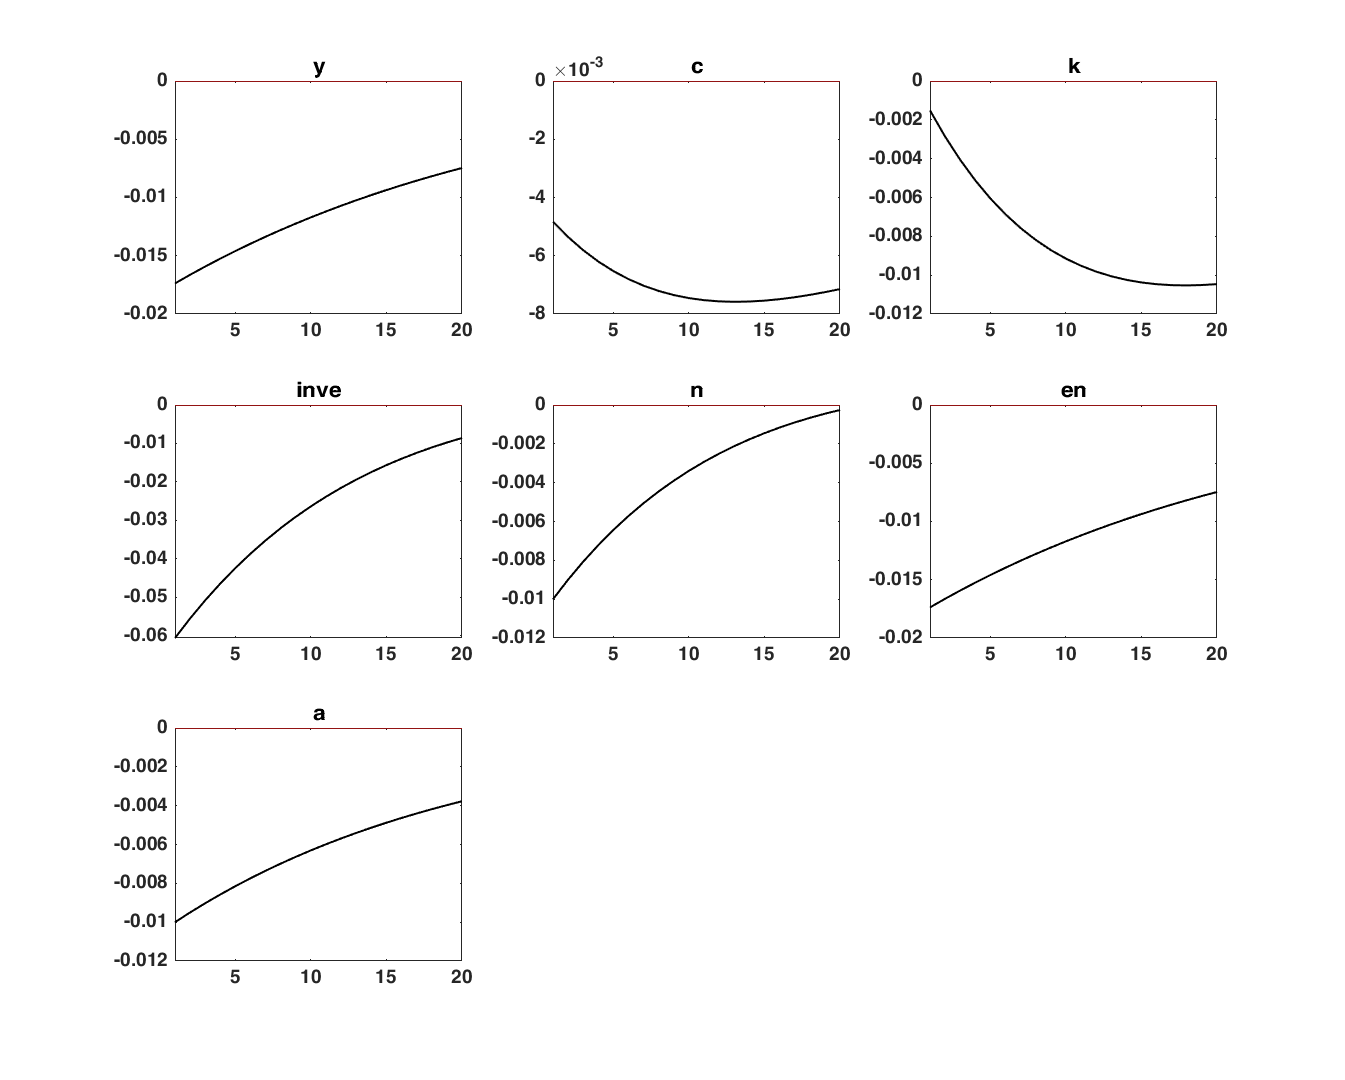
\includegraphics[scale=0.4]{IRF_ProductivityShock.png}
    \caption{Impulse Response Functions (IRF) to a negative 1\% shock to Total Factor Productivity}
    \label{fig:my_label}
\end{figure}

\textbf{Intepretation:}\\
The impulse response functions of a negative 1\%  TFP shock show the adjustment of the economy to a reduction in its productive capacity. TFP measures the efficiency with which labor and capital inputs are used to produce output in the economy. Therefore, a negative TFP shock leads to a decline in the economy's productivity, leading to a decline in output, income, consumption, and investment.\\

The impulse response functions show that the negative TFP shock leads to an immediate decline in output, which reflects the immediate reduction in the productivity of labor and capital inputs. The fall in output is persistent, indicating that the shock has long-lasting effects on the economy's productive capacity. The persistence of the decline in output is due to the slow adjustment of capital and labor inputs to the new lower level of productivity.\\

The decline in output leads to a fall in consumption, investment, and labor supply and Energy required. Consumption falls less than output because households can smooth their consumption over time by using their savings. Investment falls more than consumption because firms reduce their capital expenditures in response to the lower productivity. The fall in labor supply reflects the decrease in the economy's production capacity, as fewer workers are needed to produce the lower level of output. Also less Energy is needed to produce the lower level of output, but it declines less than the labor supply.\\

In summary, the impulse response functions of a negative TFP shock show that the shock has negative effects on the economy's output, consumption, investment, labor supply, and Energy. The persistence of the decline in output shows how long-lasting the negative effect is on the economy's productivity. The economy gradually returns to its pre-shock level.


\subsection{Positive Shock To Energy Prices}
\begin{figure}[H]
    \centering
    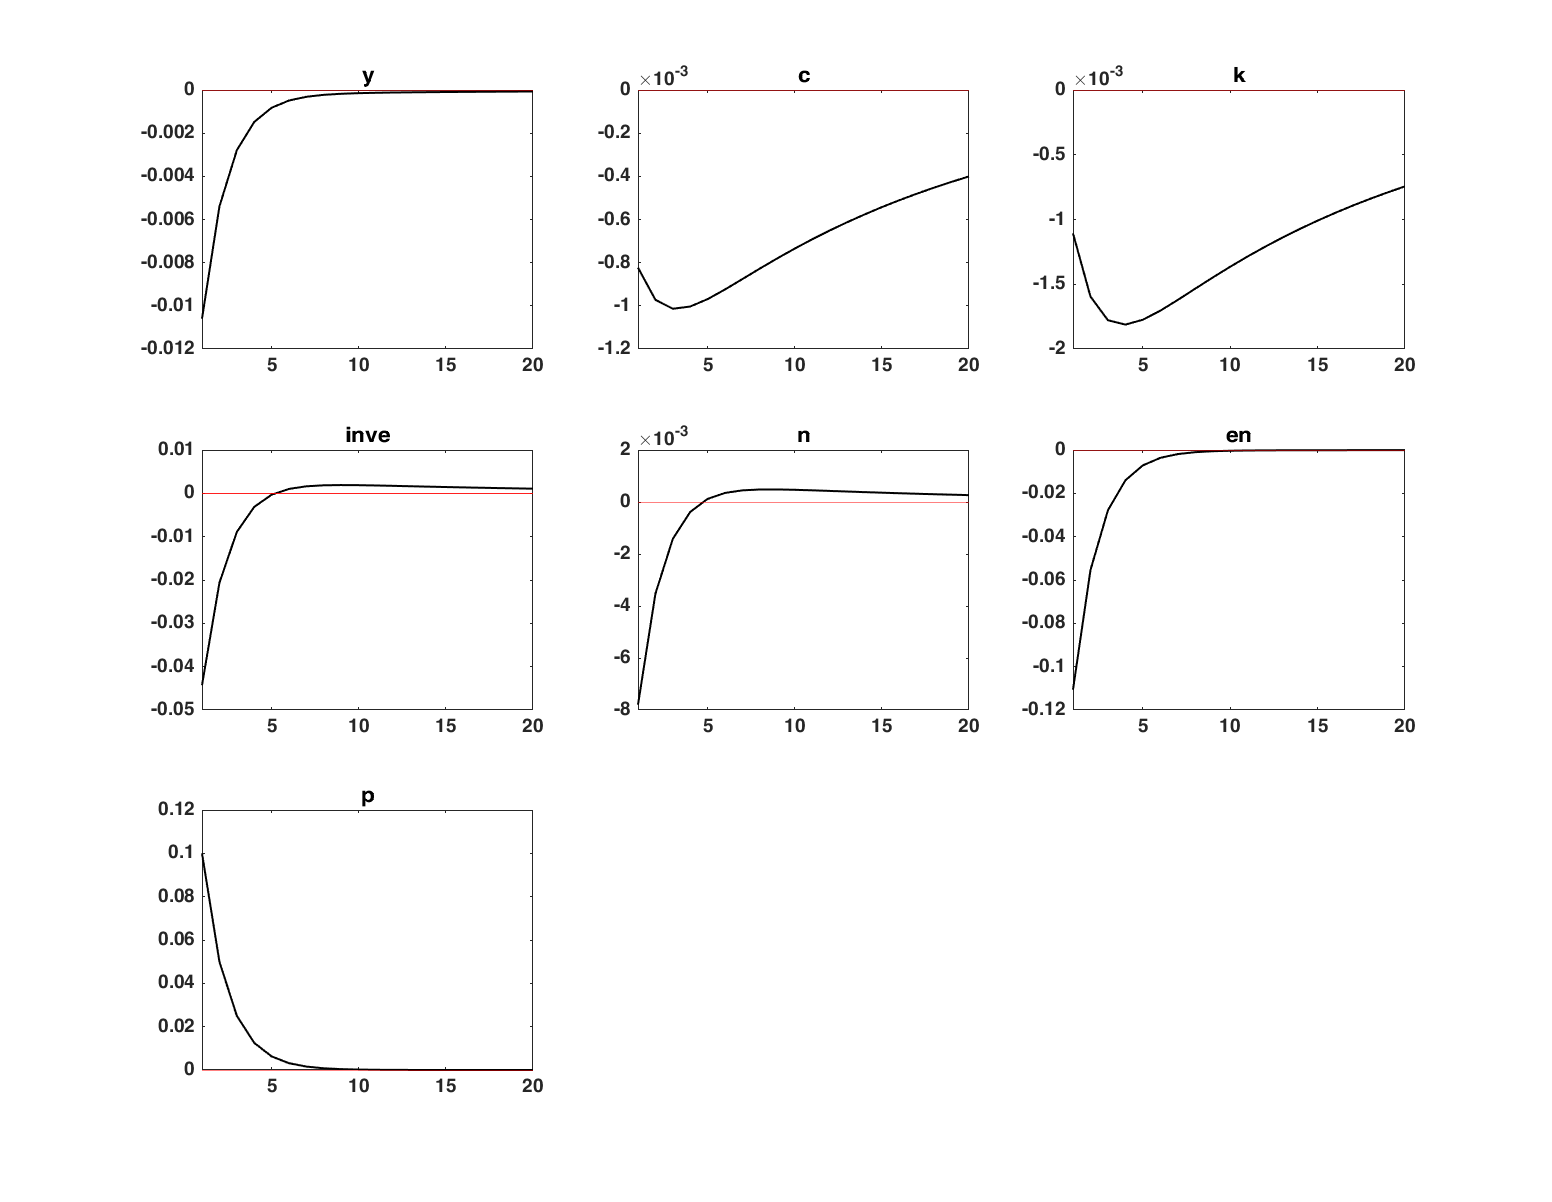
\includegraphics[scale=0.4]{IRF_EnergyShock.png}
    \caption{Impulse Response Functions (IRF) to a positive 1\% energy price shock }
    \label{fig:my_label}
\end{figure}
\pagebreak

\textbf{Interpretation:} 
The impulse response functions of a positive 1\% Energy price shock show the adjustment of the economy to an increase in the Energy price, which increases the price of Energy inputs used in production. This shock affects the production costs and leads to a change in the relative prices of goods and services in the economy.\\

The immediate effect of the energy price shock is a decline in output. The reduction in output is because the increase in energy prices leads to a rise in production costs, and firms are unable to produce the same level of output as before. The decline of Output is not very persistent and the original level of Output is reached again after a few periods. Energy declines and recovers in a similar way as Output.\\ 

The positive energy price shock leads to an immediate decline in consumption due to the rise in energy prices. Investment falls immediately following the energy price shock due to the increase in production costs, and firms' profitability is reduced. The energy price shock leads to a decline in labor supply immediately. This is because firms reduce their production, and hence, they require fewer workers to produce the same level of output.\\  

The impulse response functions of a positive energy price shock  show that the shock has a negative effect on output, consumption, investment, labor supply, and real wages in the short run. However, the economy gradually adjusts to the new higher energy prices, and the negative effects on output and other variables are not permanent.

\pagebreak
\subsection{Log-Linearization}
To gather the log-linearized version of our model we will proceed by transforming every equation in answer 2.1. The numbers refer to to the equation numbering used before.\\

\textbf{Equation 1:}\\
We rewrite in terms of the transformed variables where for some variable $X_t$ it holds that $X_t = \Bar{X}e^{\hat{X_t}}$. Thus we rewrite (1) as:\\
\begin{align*}
    & C_t^{-\sigma}A_tK_t^\alpha \gamma N_t^{\gamma-1} EN_t^{1-\alpha-\gamma}(1-N_t)=\theta\\
    & \iff C_t^{-\sigma}A_tK_t^\alpha \gamma N_t^{\gamma-1} EN_t^{1-\alpha-\gamma} - C_t^{-\sigma}A_tK_t^\alpha \gamma N_t^{\gamma} EN_t^{1-\alpha-\gamma} =\theta\\
    & \iff C_t^{-\sigma}A_tK_t^\alpha \gamma N_t^{\gamma-1} EN_t^{1-\alpha-\gamma} =\theta + C_t^{-\sigma}A_tK_t^\alpha \gamma N_t^{\gamma} EN_t^{1-\alpha-\gamma}\\
    & \iff C_t^{-\sigma}A_tK_t^\alpha \gamma N_t^{\gamma-1} EN_t^{1-\alpha-\gamma} =\theta + C_t^{-\sigma}\gamma Y_t\\
    & \iff \frac{\gamma C_t^{-\sigma} Y_t}{N_t} =\theta + C_t^{-\sigma}\gamma Y_t\\
    & \iff \gamma C_t^{-\sigma} Y_t =\theta N_t + N_t C_t^{-\sigma}\gamma Y_t\\
    & \iff C_t^{-\sigma} Y_t =\frac{\theta}{\gamma} N_t + N_t C_t^{-\sigma} Y_t\\
    &\iff \frac{Y_t}{C_t} = \frac{\theta}{\gamma}N_t + \frac{N_t Y_t}{C_t}\\
    &\iff Y_t = \frac{\theta}{\gamma}N_tC_t + N_t Y_t\\
    &\iff \Bar{Y}e^{\hat{Y_t}} = \frac{\theta}{\gamma}\Bar{N}e^{\hat{N_t}}\Bar{C}e^{\hat{C_t}} + \Bar{N}e^{\hat{N_t}} \Bar{Y}e^{\hat{Y_t}}\\
\end{align*}
Through log-linearization we thus gain
$$\Bar{Y}\hat{Y_t}= \frac{\theta}{\gamma} \Bar{C}\Bar{N}\hat{C_t} + \left(\frac{\theta}{\gamma}\Bar{C}\Bar{N} + \Bar{N}\Bar{Y}\right)\hat{N_t} + \Bar{N}\Bar{Y}\hat{Y_t}$$
\textbf{Equation 2:}\\
Using (2) from above, we use the same procedure to rewrite the right and left hand side of the equation. 
\begin{enumerate}
    \item LHS:
    \begin{align*}
        & \hat{C_t}^{-\sigma} = \Bar{C}^{-\sigma}e^{-\sigma\hat{C_t}} \simeq  \Bar{C}^{-\sigma}e^{0} -\sigma\Bar{C}^{-\sigma}(\hat{C_t}-0)
    \end{align*}
    \item RHS:
    \begin{align*}
        & \beta E_t \left[ C_{t+1}^{-\sigma}\left(A_{t+1}\alpha K_{t+1}^{\alpha-1} N_{t+1}^\gamma EN_{t+1}^{1-\alpha-\gamma}+(1-\delta)\right)\right]\\
        & = \beta E_t \left[ (\Bar{C}e^{\hat{C_{t+1}}})^{-\sigma}\left(\alpha (\Bar{A}e^{\hat{A_{t+1}}}) (\Bar{K}e^{\hat{K_{t+1}}})^{\alpha-1} (\Bar{N}e^{\hat{N_{t+1}}})^\gamma (\Bar{EN}e^{\hat{EN_{t+1}}})^{1-\alpha-\gamma}+(1-\delta)\right)\right]\\
        &\simeq \beta \left[ \Bar{C}^{-\sigma}\left(\alpha \Bar{A} \Bar{K}^{\alpha-1} \Bar{N}^\gamma \Bar{EN}^{1-\alpha-\gamma}+(1-\delta)\right)\right]\\
        &\quad +  \beta(-\sigma) \left[ \Bar{C}^{-\sigma}\left(\alpha \Bar{A} \Bar{K}^{\alpha-1} \Bar{N}^\gamma \Bar{EN}^{1-\alpha-\gamma}+(1-\delta)\right)\right]\cdot E_t[\hat{C_{t+1}}]\\
        &\quad + \beta \left[ \Bar{C}^{-\sigma}\left(\alpha \Bar{A} \Bar{K}^{\alpha-1} \Bar{N}^\gamma \Bar{EN}^{1-\alpha-\gamma}\right)\right]\cdot E_t[\hat{A_{t+1}}]\\
        &\quad + \beta (\alpha - 1) \left[ \Bar{C}^{-\sigma}\left(\alpha \Bar{A} \Bar{K}^{\alpha-1} \Bar{N}^\gamma \Bar{EN}^{1-\alpha-\gamma}\right)\right]\cdot E_t[\hat{K_{t+1}}]\\
        &\quad + \beta \gamma \left[ \Bar{C}^{-\sigma}\left(\alpha \Bar{A} \Bar{K}^{\alpha-1} \Bar{N}^\gamma \Bar{EN}^{1-\alpha-\gamma}\right)\right]\cdot E_t[\hat{N_{t+1}}]\\
        &\quad + \beta (1-\gamma-\alpha) \left[ \Bar{C}^{-\sigma}\left(\alpha \Bar{A} \Bar{K}^{\alpha-1} \Bar{N}^\gamma \Bar{EN}^{1-\alpha-\gamma}\right)\right]\cdot E_t[\hat{EN_{t+1}}]\\
    \end{align*}
    Now, we can combine the LHS with the RHS. Also, we can further simplify the equation by substracting the steady state from both sides twice and by using the fact that $\alpha \Bar{A} \Bar{K}^{\alpha-1} \Bar{N}^\gamma \Bar{EN}^{1-\alpha-\gamma} = [1-\beta(1-\delta)]$. This leaves us with the log-linearized equation:
    $$-\sigma\hat{C_t} = E_t[-\sigma\hat{C_{t+1}}+[1-\beta(1-\delta)][\hat{A_{t+1}}+(\alpha-1)\hat{K_{t+1}}+\gamma \hat{N_{t+1}}+(1-\alpha-\gamma)\hat{EN_{t+1}}]$$
\end{enumerate}
\textbf{Equation 3:}\\
Equation (3) is given by
$$P_t = A_tK_t^\alpha N_t^\gamma (1-\alpha-\gamma)EN_t^{-\alpha-\gamma}$$
Using (6) this can be rewritten as 
$$P_t = \frac{Y_t}{EN_t}(1-\alpha-\gamma) \iff EN_t P_t = Y_t(1-\alpha-\gamma)$$
We now rewrite this as deviations and gain
$$\Bar{EN}e^{\hat{EN_t}} \Bar{P}e^{\hat{P_t}} = \Bar{Y}e^{\hat{Y_t}}(1-\alpha-\gamma)$$
By using log-linearization on both sides (LHS = RHS) we get our log-linearized version as
\begin{align*}
    &\Bar{P}\Bar{EN} + \Bar{P}\Bar{EN}(\hat{P_t} + \hat{EN_t}) = \Bar{Y}(1-\alpha-\gamma) + \Bar{Y}(1-\alpha-\gamma)\hat{Y_t}\\
    &\iff \Bar{P}\Bar{EN}\hat{P_t} + \Bar{P}\Bar{EN}\hat{EN_t} =  \Bar{Y}(1-\alpha-\gamma)\hat{Y_t}
\end{align*}
\textbf{Equation 4:}\\
Due the linear structure of the resource constraint, we can see that 
$$ A_tK_t^\alpha N_t^\gamma EN_t^{1-\alpha-\gamma} + (1-\delta)K_t = C_t + K_{t+1}+P_tEN_t $$
rewritten with the transformed variables yields
$$(\Bar{A}e^{\hat{a_t}})(\Bar{K}e^{\hat{K_t}})^\alpha(\Bar{N}e^{\hat{N_t}})^\gamma (\Bar{EN}e^{\hat{EN_t}})^{(1-\alpha-\gamma)} + (1-\delta)\Bar{K}e^{\hat{K_t}} = \Bar{C}e^{\hat{C_t}} + \Bar{K}e^{\hat{K_{t+1}}} + \Bar{P}e^{\hat{P_t}}\Bar{EN}e^{\hat{EN_t}}$$
\begin{itemize}
    \item RHS $\simeq \Bar{C} + \Bar{K} + \Bar{P}\Bar{EN} + \Bar{C}\hat{C_t} +\Bar{K}\hat{K_{t+1}} + \Bar{P}\Bar{EN}(\hat{P_t} + \hat{EN_t})$
    \item LHS $\simeq$ \begin{align*}
        &\Bar{A} \Bar{K}^{\alpha} \Bar{N}^\gamma \Bar{EN}^{1-\alpha-\gamma}+(1-\delta)\Bar{K} \\
        &\quad + \alpha \Bar{A} \Bar{K}^{\alpha-1} \Bar{N}^\gamma \Bar{EN}^{1-\alpha-\gamma}\hat{A_{t}}\\
        &\quad + [\alpha \Bar{A} \Bar{K}^{\alpha-1} \Bar{N}^\gamma \Bar{EN}^{1-\alpha-\gamma}+(1-\delta)\Bar{K}]\hat{K_t}\\
        &\quad + (1-\alpha-\gamma) \Bar{A} \Bar{K}^{\alpha-1} \Bar{N}^\gamma \Bar{EN}^{1-\alpha-\gamma}\hat{EN_t}\\
        &\quad + \gamma \Bar{A} \Bar{K}^{\alpha-1} \Bar{N}^\gamma \Bar{EN}^{1-\alpha-\gamma}\hat{N_t}
    \end{align*}
\end{itemize}
Setting LHS = RHS, substracting the steady state from both sides and dividing by $\Bar{Y}$ yields the final equation
$$\frac{\Bar{C}}{\Bar{Y}}\Hat{C_t} + \frac{\Bar{K}}{\Bar{Y}}\Hat{K_{t+1}} + \frac{\Bar{P}\Bar{EN}}{\Bar{Y}}(\Hat{P_t} + \Bar{EN_t}) = \hat{A_t} + \alpha \hat{K_t} + (1-\alpha-\gamma)\hat{EN_t} + \gamma\hat{N_t} + (1-\delta)\frac{\Bar{K}}{\Bar{Y}}\hat{K_t}$$
\textbf{Equation 5:}
We continue by examining equation (5), which is given by and can be rewritten as 
$$I_t = K_{t+1} - (1-\delta)K_t \implies \Bar{I}e^{\hat{I_{t+1}}} = \Bar{K}e^{\hat{K_{t+1}}} - (1- \delta)\Bar{K}e^{\hat{K_{t}}}$$
Using log-linearization we can gain
$$\Bar{I} + \Bar{I}\hat{I_t} = \Bar{K}-(1-\delta)\Bar{K} + \Bar{K}\hat{K_{t+1}}-(1-\delta)\Bar{K}\hat{K_{t}}$$
$$\iff \Bar{I}\hat{I_t} = \Bar{K}\hat{K_{t+1}}-(1-\delta)\Bar{K}\hat{K_{t}}$$
\textbf{Equation 6:}
The next equation (6) is given by
    $$Y_t = A_tK_t^\alpha N_t^\gamma EN_t^{1-\alpha-\gamma}$$
Rewriting it as usual yields
    $$\Bar{Y}e^{\hat{Y_t}} = \Bar{A}e^{\hat{A_t}}(\Bar{K}e^{\hat{K_t}})^\alpha (\Bar{N}e^{\hat{N_t}})^\gamma (\Bar{EN}e^{\hat{EN_t}})^{1-\alpha-\gamma}$$
Expanding around the steady state results in
$$LHS \simeq \Bar{Y} + \Bar{Y}\hat{Y_t}$$
as well as
\begin{align*}
	&RHS \simeq \Bar{A} \Bar{K}^{\alpha} \Bar{N}^\gamma \Bar{EN}^{1-\alpha-\gamma}\\
	&\quad + \Bar{A} \Bar{K}^{\alpha} \Bar{N}^\gamma \Bar{EN}^{1-\alpha-\gamma}\hat{A_t}\\
	&\quad + \alpha \Bar{A} \Bar{K}^{\alpha} \Bar{N}^\gamma \Bar{EN}^{1-\alpha-\gamma}\hat{K_t}\\
	&\quad + \gamma \Bar{A} \Bar{K}^{\alpha} \Bar{N}^\gamma \Bar{EN}^{1-\alpha-\gamma}\hat{N_t}\\
	&\quad + (1-\alpha-\gamma) \Bar{A} \Bar{K}^{\alpha} \Bar{N}^\gamma \Bar{EN}^{1-\alpha-\gamma}\hat{EN_t}\\
\end{align*}
Setting LHS equal to RHS and substracting the steady state yields
$$\Bar{Y}\hat{Y_t} = \Bar{A} \Bar{K}^{\alpha} \Bar{N}^\gamma \Bar{EN}^{1-\alpha-\gamma}\hat{A_t} + \cdots + (1-\alpha-\gamma) \Bar{A} \Bar{K}^{\alpha} \Bar{N}^\gamma \Bar{EN}^{1-\alpha-\gamma}\hat{EN_t}$$
$$\iff \hat{Y_t} = \hat{A_t} + \alpha \hat{K_t} + \gamma \hat{N_t} + (1-\alpha-\gamma)\hat{EN_t}$$
Equations (7) and (8) are already in log-linearized form, thus we can write:\\
\textbf{Equation 7:}\\
    $$\log(A_{t+1}) = \rho_A \log(A_{t}) + \epsilon_{A,t+1}$$

\textbf{Equation 8:}\\
    $$\log(P_{t+1}) = \rho_P \log(P_{t}) + \epsilon_{P,t+1}$$

which completes our set of log-linearized equations.

\subsection{Matrix Modelling}
Using the previously derived equations, we can setup matrices A and B which satisfy the relationship
$$A\cdot E_t z_{t+1} = B z_t$$
where $z_t = [\hat{K_t} \quad \hat{A_t} \quad \hat{P_t} \quad  \hat{C_t} \quad \hat{I_t} \quad \hat{Y_t} \quad \hat{N_t} \quad \hat{EN_t}]^T$.
The matrices which will be used to solve the system using the Klein algorithm look like
$$A = \begin{bmatrix}
0&0&0&0&0&0&0&0\\
[1-\beta(1-\delta)](\alpha-1)&[1-\beta(1-\delta)]&0&-\sigma&0&0&[1-\beta(1-\delta)]\gamma&[1-\beta(1-\delta)](1-\gamma-\alpha)\\
0&0&0&0&0&0&0&0\\
\bar{K}/\bar{Y}&0&0&0&0&0&0&0\\
\bar{K}&0&0&0&0&0&0&0\\
0&0&0&0&0&0&0&0\\
0&1&0&0&0&0&0&0\\
0&0&1&0&0&0&0&0\\
\end{bmatrix}$$
as well as
$$B = \begin{bmatrix}
0&0&0&\frac{\theta}{\gamma}\bar{C}\bar{N}&0&-\bar{Y}+\bar{N}\bar{Y}&\bar{N}(\frac{\theta}{\gamma}\bar{C}+\bar{Y})&0\\
0&0&0&-\sigma&0&0&0&0\\
0&0&\bar{P}\bar{EN}&0&0&-\bar{Y}(1-\alpha-\gamma)&0&\bar{P}\bar{EN}\\
\alpha+(1-\delta)\frac{\bar{K}}{\bar{Y}} &1&-\frac{\bar{P}\bar{EN}}{\bar{Y}}&-\frac{\bar{C}}{\bar{Y}}&0&0&\gamma&-\frac{\bar{P}\bar{EN}}{\bar{Y}}+1-\alpha-\gamma\\
(1-\delta)\bar{K}&0&0&0&\bar{I}&0&0&0\\
-\alpha &-1 &0&0&0&1&-\gamma &-(1-\alpha-\gamma)\\
0&\rho_A &0&0&0&0&0&0\\
0&0&\rho_P &0&0&0&0&0\\
\end{bmatrix}$$
Again, our code file can be found on \href{https://github.com/therealLucasPaul/AdvMacroeconomics2_Assignments}{GitHub} or in the appendix. The computed matrices \textbf{G} and \textbf{H} can be found below:

$$H = \begin{bmatrix}
    0.941  &  0.1515 &  -0.0111 \\
    0  &  0.9500  &  0 \\
   0  &  0   & 0.5 \\
\end{bmatrix} \quad G = \begin{bmatrix}
   -1.3589  &  6.0581 &  -0.4428 \\
    0.0868  &  1.7370 &  -0.1060 \\
    0.5064  &  0.4831 &  -0.0082 \\
   -0.3346  &  1.0002 &  -0.0780 \\
    0.0868  &  1.7370 &  -1.1060 \\
\end{bmatrix}$$
These matrices represent the following matrices:
$$H = \begin{bmatrix}
    \phi_{kk}  &  \phi_{ka} &  \phi_{kp} \\
    0  &  \rho_p  &  0 \\
   0  &  0   & \rho_a \\
\end{bmatrix} \quad G = \begin{bmatrix}
    \phi_{ik} &  \phi_{ia} &  \phi_{ip} \\
    \phi_{yk} &  \phi_{ya} &  \phi_{yp} \\
    \phi_{ck} &  \phi_{ca} &  \phi_{cp} \\
    \phi_{nk} &  \phi_{na} &  \phi_{np} \\
    \phi_{enk} &  \phi_{ena} &  \phi_{enp} \\
\end{bmatrix}$$

Thus, all in all the system looks like
$$\begin{bmatrix}
    \hat{i}_t \\
    \hat{y}_t \\
    \hat{c}_t \\
    \hat{n}_t \\
    \hat{en}_t \\
\end{bmatrix} = \begin{bmatrix}
    \phi_{ik} &  \phi_{ia} &  \phi_{ip} \\
    \phi_{yk} &  \phi_{ya} &  \phi_{yp} \\
    \phi_{ck} &  \phi_{ca} &  \phi_{cp} \\
    \phi_{nk} &  \phi_{na} &  \phi_{np} \\
    \phi_{enk} &  \phi_{ena} &  \phi_{enp} \\
\end{bmatrix} \cdot \begin{bmatrix}
    \hat{k}_t \\
    \hat{a}_t \\
    \hat{p}_t 
\end{bmatrix}$$
which corresponds with our previously reported policy values.
\pagebreak
\section{Appendix}
\subsection{Dynare Code for question 3(b)}
\lstinputlisting[language=Matlab]{Assignment1_Dynare.mod}

\pagebreak
\subsection{Matlab Code for question 3(f)}
\lstinputlisting[language=Matlab]{Assignment1_QuestionF.m}
\end{document}
